\documentclass[11pt]{beamer}
\usepackage[utf8]{inputenc}
\usepackage{graphicx, epsfig}
\usepackage{amsmath,mathrsfs,amsfonts,amssymb}
%\usepackage{subfig}
\usepackage{floatflt}
\usepackage{epic,ecltree}
\usepackage{mathtext}
\usepackage{fancybox}
\usepackage{fancyhdr}
\usepackage{multirow}
\usepackage{enumerate}
\usepackage{epstopdf}
\usepackage{multicol}
\usepackage{algorithm}
\usepackage[noend]{algorithmic}
\usepackage{tikz}
\usepackage{blindtext}
\usetheme{default}%{default}%{Singapore}%{Warsaw}%{Warsaw}%{Darmstadt}
\usecolortheme{default}
\setbeamerfont{title}{size=\Huge}
\setbeamertemplate{footline}[page number]{}


\makeatletter
\newcommand\HUGE{\@setfontsize\Huge{35}{40}}
\makeatother    

\setbeamerfont{title}{size=\HUGE}
\beamertemplatenavigationsymbolsempty

% latin bold lower
\newcommand{\ba}{\mathbf{a}} 
\newcommand{\bc}{\mathbf{c}} 
\newcommand{\be}{\mathbf{e}} 
\newcommand{\bh}{\mathbf{h}} 
\newcommand{\bp}{\mathbf{p}} 
\newcommand{\bt}{\mathbf{t}} 
\newcommand{\bs}{\mathbf{s}} 
\newcommand{\bu}{\mathbf{u}} 
\newcommand{\bv}{\mathbf{v}} 
\newcommand{\bw}{\mathbf{w}} 
\newcommand{\bx}{\mathbf{x}} 
\newcommand{\by}{\mathbf{y}} 
\newcommand{\bz}{\mathbf{z}} 

% latin bold upper
\newcommand{\bA}{\mathbf{A}} 
\newcommand{\bB}{\mathbf{B}} 
\newcommand{\bC}{\mathbf{C}} 
\newcommand{\bI}{\mathbf{I}} 
\newcommand{\bL}{\mathbf{L}} 
\newcommand{\bM}{\mathbf{M}} 
\newcommand{\bQ}{\mathbf{Q}} 
\newcommand{\bT}{\mathbf{T}} 
\newcommand{\bU}{\mathbf{U}} 
\newcommand{\bV}{\mathbf{V}} 
\newcommand{\bW}{\mathbf{W}} 
\newcommand{\bX}{\mathbf{X}} 
\newcommand{\bY}{\mathbf{Y}} 
\newcommand{\bZ}{\mathbf{Z}} 

% latin cal upper
\newcommand{\cG}{\mathcal{G}} 
\newcommand{\cL}{\mathcal{L}} 
\newcommand{\cN}{\mathcal{N}} 
\newcommand{\cS}{\mathcal{S}} 
\newcommand{\cT}{\mathcal{T}} 
\newcommand{\cW}{\mathcal{W}} 
\newcommand{\cX}{\mathcal{X}} 
\newcommand{\cZ}{\mathcal{Z}} 

% latin bb upper
\newcommand{\bbE}{\mathbb{E}} 
\newcommand{\bbI}{\mathbb{I}} 
\newcommand{\bbP}{\mathbb{P}} 
\newcommand{\bbR}{\mathbb{R}} 

% greek bold lower
\newcommand{\bepsilon}{\boldsymbol{\epsilon}} 
\newcommand{\btheta}{\boldsymbol{\theta}} 
\newcommand{\blambda}{\boldsymbol{\lambda}} 
\newcommand{\bpi}{\boldsymbol{\pi}} 
\newcommand{\bmu}{\boldsymbol{\mu}} 
\newcommand{\bsigma}{\boldsymbol{\sigma}} 
\newcommand{\bphi}{\boldsymbol{\phi}} 

% greek bold upper
\newcommand{\bSigma}{\boldsymbol{\Sigma}} 

\DeclareMathOperator*{\argmin}{arg\,min}
\DeclareMathOperator*{\argmax}{arg\,max}
\newcommand{\createdgmtitle}[1]{\title[\hbox to 56mm{Mathematical Forecasting Methods \hfill\insertframenumber\,/\,\inserttotalframenumber}]
	{\vspace{1.5\cm} \\ Mathematical Forecasting Methods \\ {\Huge Лекция #1}}
	\author{}
	\institute{
	МФТИ
	} 
	\date{Осень, 2023}
}

\newcommand\myfootnote[1]{%
  \tikz[remember picture,overlay]
  \draw (current page.south west) +(1in + \oddsidemargin,0.5em)
  node[anchor=south west,inner sep=0pt]{\parbox{\textwidth}{%
      \rlap{\rule{10em}{0.4pt}}\raggedright\scriptsize \textit{#1}}};}

\newcommand\myfootnotewithlink[2]{%
  \tikz[remember picture,overlay]
  \draw (current page.south west) +(1in + \oddsidemargin,0.5em)
  node[anchor=south west,inner sep=0pt]{\parbox{\textwidth}{%
      \rlap{\rule{10em}{0.4pt}}\raggedright\scriptsize\href{#1}{\textit{#2}}}};}
\createdgmtitle{6}
\usepackage{tikz}
\usepackage{amsmath}
\usepackage[english,russian]{babel}
\usepackage[labelformat=empty]{caption}

\usepackage{graphicx,animate}
\usepackage{animate}

\usetikzlibrary{arrows,shapes,positioning,shadows,trees}
\newcommand*{\defeq}{\stackrel{\text{def}}{=}}

%--------------------------------------------------------------------------------
\begin{document}
%--------------------------------------------------------------------------------
\begin{frame}[plain]
%\thispagestyle{empty}
\titlepage
\end{frame}
%=======
\begin{frame}{Краткое повторение}
\begin{itemize}
    \item Математические основы динамических систем позволяют осуществлять анализ временных рядов.
    \item Теорема Такенса позволяет использовать вектора задержек для восстановления внутренней структуры динамической системы.
    \item При выполнении условия $m \geq 2d + 1$, где $d$ — размерность вложения, возможно реконструировать пространство состояний системы.
    \item В частности, выводы теоремы Такенса используются в CCM. Алгоритм CCM является аналогом статистического теста и оценивает причинно-следственную связь двух временных рядов.
\end{itemize}
\end{frame}
%=======
\begin{frame}{Краткое повторение}
\begin{figure}
    \centering
    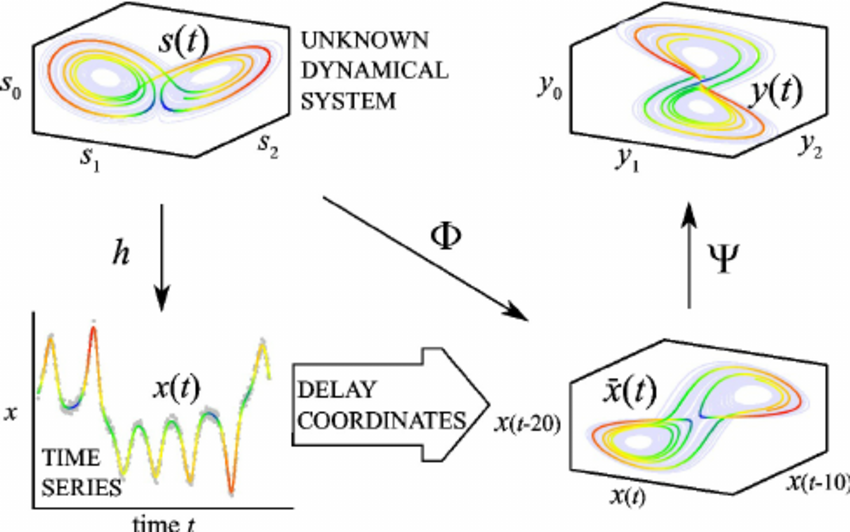
\includegraphics[width=\textwidth]{lecture_5/figs/CCM-1.png}
\end{figure}
\end{frame}
%=======
\begin{frame}{Cross Convergent Mapping}
\begin{figure}
    \centering
    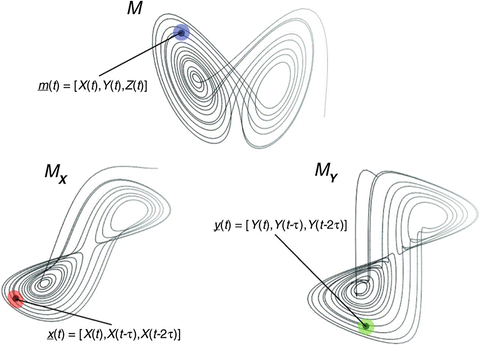
\includegraphics[width=\textwidth]{lecture_5/figs/CCM.png}
\end{figure}
\end{frame}
%=======
\begin{frame}{Краткое повторение}

\begin{enumerate}
    \item Пусть имеются 2 временных ряда $\{x_1, x_2,...,x_T\}$ и $\{y_1, y_2,...,y_T\}$ длины $T$.
    \item Для ряда $\{x_t\}_{t=1}^T$ формируем векторы предыстории размерности $E$ с шагом по времени $\tau$:
    $$ \mathbf{x}_t = \begin{pmatrix}
        x_t, & x_{t - \tau}, & x_{t - 2\tau}, & \dots, & x_{t - (E-1)\tau}
    \end{pmatrix}$$
    \item В пространстве $\mathbb{R}^E$ (\textit{фазовом пространстве}) такие векторы предыстории образуют\textit{фазовую траекторию} системы -- множество $M_x = \{\mathbf{x}_t \ | \ t = 1 + (E - 1)\tau, ..., T \}$.
    \item[4.] Пусть требуется построить предсказание для значения $y_t$. Для этого сначала найдем $E + 1$ векторов из $M_x$, ближайших к $\mathbf{x}_t$ (в терминах, например, стандартной метрики $d$ в $\mathbb{R}^n$). Пусть им соответствуют временные индексы $t_1, ..., t_{E+1}$, отсортированные в порядке от ближайшей точки до наиболее удалённой.
    $$ d_i = d(\mathbf{x}_t, \mathbf{x}_{t_i}), \quad d_1 < d_2 < ... < d_{E + 1}$$
\end{enumerate}

\end{frame}
%=======

\begin{frame}{Алгоритм Convergent Cross Mapping}

\begin{enumerate}

    \item[5.] Тогда оценка значения $y_t$ строится следующим образом в виде взвешенной суммы значений ряда в моменты времени $t_1, ..., t_{E+1}$:
    $$ \hat{y}_t|M_x = \sum_{i=1}^{E+1} \omega_i y(t_i)$$
    $$ \omega_i = \frac{u_i}{\displaystyle \sum_{j=1}^{E + 1}u_j}, \quad \quad u_i = \text{exp}\Big(-\frac{d_i}{d_1}\Big), \quad \quad i = 1, ..., E+1$$
    \item[6.] Для того, чтобы посудить о существовании зависимости между рядами $\{x_t\}_{t=1}^T$ и $\{у_t\}_{t=1}^T$, рассчитаем теперь коэффициент корреляции Пирсона:
    $$ C_{yx} = \Bigg[\rho \Big( y, \hat{y}|M_x \Big) \Bigg]^2$$

\end{enumerate}

\end{frame}
%=======
\begin{frame}{Применение рядов Фурье для анализа временных рядов}
Исследуется функция $x(t)$, заданная на отрезке $[0, T]$.\newline
Фурье-анализ позволяет представить функцию $x(t)$ в виде:

$$x(t) = a_0 + \sum_{k=1}^{+\infty}a_k \text{cos}(2\pi\frac{k}{T}t + \theta_k)$$

$T$ -- отрезок, где функция определена (длительность сигнала)\\
$a_k$ -- амплитуда $k$-ой гармонической составляющей,\\
$\theta_k$ -- начальная фаза $k$-ой гармонической составляющей.
\vspace{0.5cm}

Разложение в ряд Фурье позволяет представить непрерывную функцию $x(t)$, определенную на отрезке $[0, T]$ в виде бесконечного ряда тригонометрических функций с определёнными амплитудами и фазами, также рассматриваемых на отрезке $[0, T]$.

\end{frame}
%=======
\begin{frame}{Применение рядов Фурье для анализа временных рядов}
\begin{figure}
    \centering
    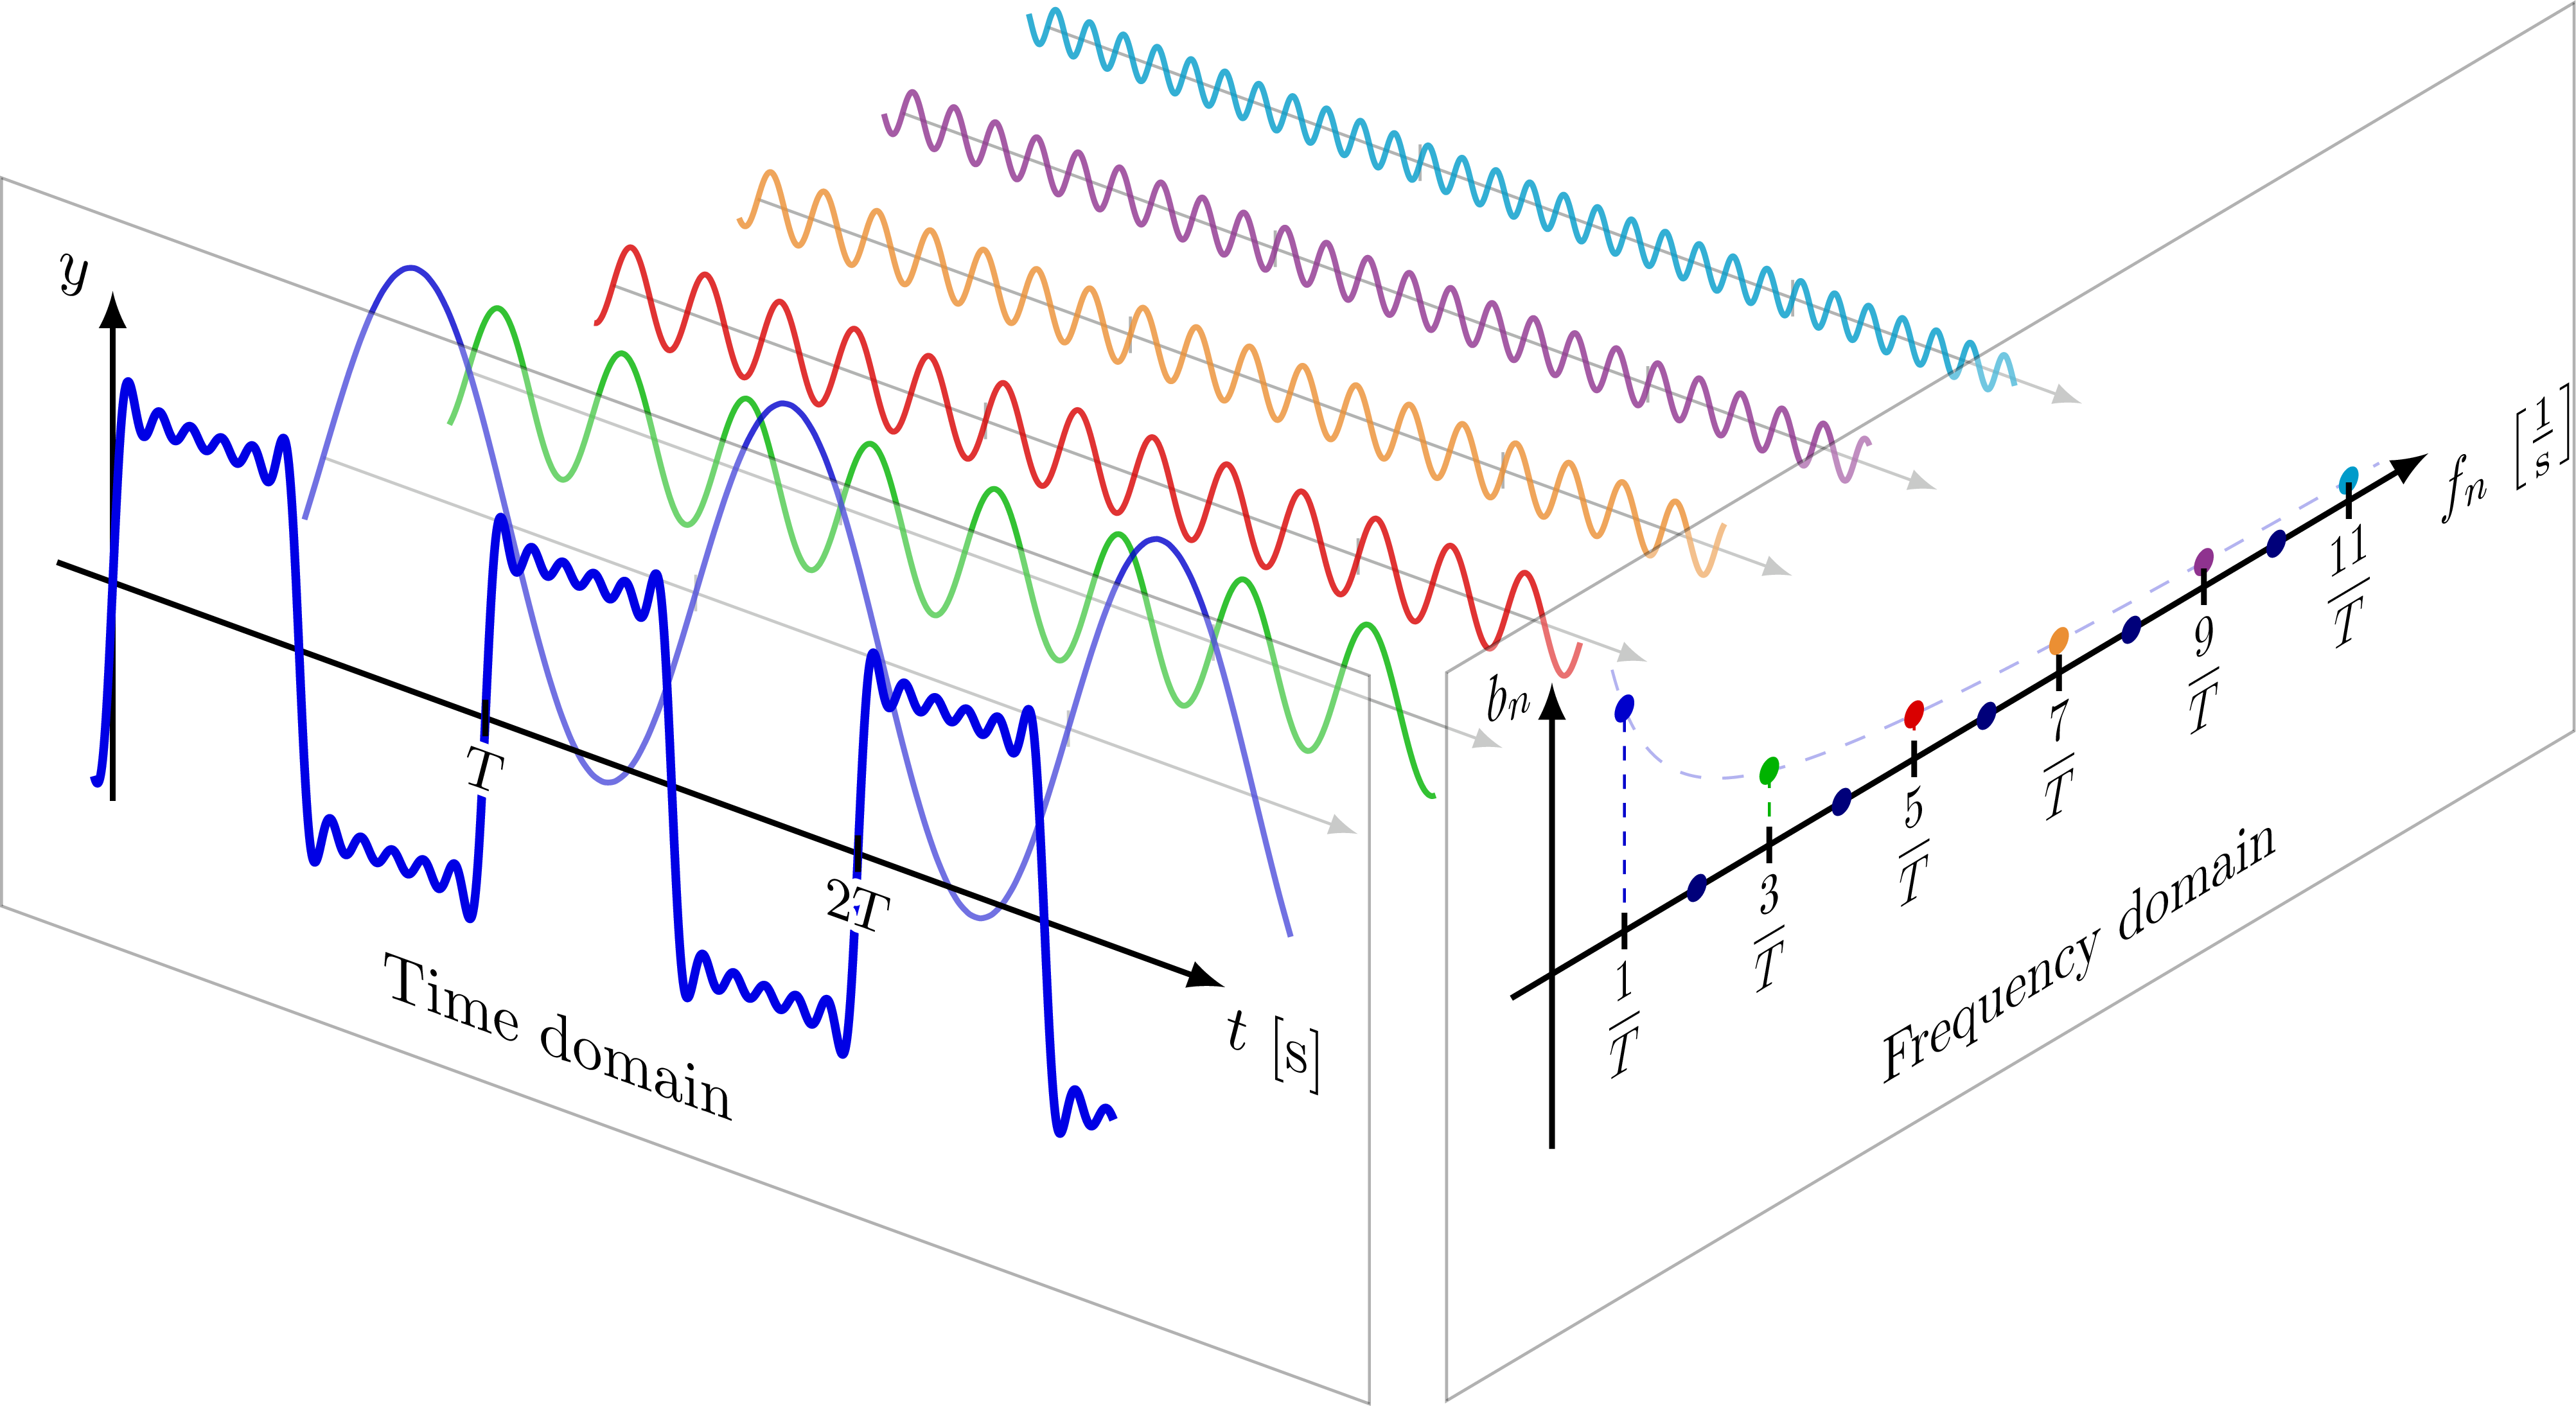
\includegraphics[width=\textwidth]{lecture_6/fourier_series_2.png}
\end{figure}
\end{frame}
%=======
\begin{frame}{Глобальные и локальные методы прогнозирования}
В анализе и прогнозировании временных рядов можно выделить две группы методов:
\begin{itemize}
    \item глобальные -- параметры аппроксимирующей функции находятся посредством использования всех известных значений ряда; основное приложение -- получение глобальных характеристик
    системы (ARMA, SSA)
    \item локальные методы основаны на принципе локальной аппроксимации (LA)
\end{itemize}
\end{frame}

\begin{frame}{Глобальные и локальные методы прогнозирования}
Преимущества локальных методов прогноза нерегулярных (хаотических, квазипериодических) рядов:
\begin{itemize}
    \item применение не требует априорной информации о системе, породившей временной ряд
    \item нет необходимости в построении специфической модели динамики исследуемого ряда
    \item использования для прогнозирования наиболее близких к стартовой
точке (стартовому вектору) значений ряда
    \item использование меньшего количества исходных данных
    \item меньше ограничений на горизонт прогнозирования
\end{itemize}

\end{frame}
%=======

\begin{frame}{Матричное представление временного ряда}
\begin{itemize}
    \item Вектор задержек: 
    $$ \mathbf{x}_t = (x_t, x_{t+1}, \dots, x_{t + \tau - 1})^T \in \mathbb{R}^{\tau}$$
    \item Матрица задержек:
    $$\mathbf{X} = 
    \begin{pmatrix}
    \mathbf{x}_1 & \mathbf{x}_2 & \mathbf{x}_3 & \dots & \mathbf{x}_{\tau} & \dots & \mathbf{x}_n
    \end{pmatrix} = $$
    $$ = \begin{pmatrix}
    x_1 & x_2 & x_3 & \dots & x_{\tau} & \dots & x_n \\
    x_2 & x_3 & x_4 & \dots & x_{\tau + 1} & \dots & x_{n + 1} \\
    x_3 & x_4 & x_5 & \dots & x_{\tau + 2} & \dots & x_{n + 2} \\
    \vdots & \vdots & \vdots & \ddots & \vdots & \ddots & \vdots \\
    x_{\tau} & x_{\tau + 1} & x_{\tau + 2} & \dots & x_{2\tau - 1} & \dots & x_N 
    \end{pmatrix} \in \mathbb{R}^{\tau \times n}$$
    Здесь предполагаем, что $n > \tau$.
\end{itemize}
\end{frame}
%=======
\begin{frame}{SVD: напоминание}
    Для матрицы $\mathbf{X}$ существует (и, вообще говоря, не единственно) сингулярное разложение:
    $$ \underset{\tau \times n}{\mathbf{X}} = \underset{\tau \times \tau}{U} \ \underset{\tau \times n}{\Sigma} \ \underset{n \times n}{V^T}$$
    Здесь:
    \begin{itemize}
        \item $U \in \mathbb{R}^{\tau \times \tau}$ -- ортогональная матрица собств. векторов $\mathbf{X}\mathbf{X}^T$ (столбцы $U$ образуют ортонормированный базис в $\mathbb{R}^{\tau}$)
        \item $\Sigma \in \mathbb{R}^{\tau \times n}$ -- прямоугольная диагональная матрица сингулярных чисел $\mathbf{X}$, причем $\sigma_1 \geq \sigma_2 \geq \dots \geq \sigma_{\tau}$:
        $$ \Sigma = \begin{pmatrix}
            \sigma_1  & \dots & 0 & 0 & \dots & 0 \\
            \vdots  & \ddots & \vdots & \vdots & \dots & \vdots \\
            0 &  \dots & \sigma_{\tau} & 0 & \dots & 0
        \end{pmatrix}$$
        \item $V \in \mathbb{R}^{n \times n}$ -- ортогональная матрица собств. векторов $\mathbf{X}^T\mathbf{X}$ (столбцы $V$ образуют ортонормированный базис в $\mathbb{R}^{n}$)
    \end{itemize}
\end{frame}
%=======

\begin{frame}{Low Rank Approximation}
    Одним из важных свойств сингулярного разложения матрицы является возможность построения для неё \textit{низкорангового приближения}, а именно:
    \begin{itemize}
        \item Пусть $A \in \mathbb{R}^{m \times n}$, $ A = U \Sigma V^T$ -- сингулярное разложение $A$.
        \item Рассмотрим матрицу $\Sigma$ и её приближение ранга $r$ -- матрицу $\tilde{\Sigma}$, где подматрица $\Sigma_1$ имеет размер $r \times r$:
        $$ \Sigma = 
        \begin{bmatrix}
        \Sigma_1 & 0 \\
        0 & \Sigma_2
        \end{bmatrix}, \quad 
        \tilde{\Sigma} = 
        \begin{bmatrix}
        \Sigma_1 & 0 \\
        0 & 0
        \end{bmatrix}$$
        \item \textbf{Теорема:} среди всех матриц $B$ ранга не более $r$ норма разности матриц $A$ и $\tilde{A} = U \tilde{\Sigma} V^T$ минимальна: 
        $$\tilde{A} = \argmin_{\text{rank}(B) \leq r}{|| A - B ||} \quad \text{(верно для $|| \cdot ||_2$, для $|| \cdot ||_F$)}$$
        
        \item Матрица $\tilde{A}$ также может быть получена, как $\tilde{A} = U_1 \Sigma_1 V_1^T$, где $U_1, \ V_1$ -- первые $r$ столбцов матриц $U$ и $V$.
        
    \end{itemize}
\end{frame}
%=======
\begin{frame}{Метод SSA и алгоритм SSA-сглаживания}
Метод SSA (Singular Spectral Analysis) основан на использовании сингулярного разложения матрицы задержек для анализа временного ряда.\\
\textbf{Алгоритм SSA-сглаживания:}
\begin{enumerate}
    \item Для матрицы задержек $\mathbf{X}$ построим её низкоранговое приближение $\tilde{\mathbf{X}}$ с помощью SVD.
    \item Из элементов матрицы $\tilde{\mathbf{X}}$ получим cглаженные оценки значений временного ряда $x_1, ..., x_N$. Заметим, что в исходной матрице эти значения стоят на нескольких позициях одновременно:
    $$ \mathbf{X} = \begin{pmatrix}
    \textcolor{red}{x_1} & \textcolor{orange}{x_2} & \textcolor{yellow}{x_3} & \dots & x_{\tau} & \dots & x_n \\
    \textcolor{orange}{x_2} & \textcolor{yellow}{x_3} & \textcolor{green}{x_4} & \dots & x_{\tau + 1} & \dots & x_{n + 1} \\
    \textcolor{yellow}{x_3} & \textcolor{green}{x_4} & \textcolor{cyan}{x_5} & \dots & x_{\tau + 2} & \dots & x_{n + 2} \\
    \vdots & \vdots & \vdots & \ddots & \vdots & \ddots & \vdots \\
    x_{\tau} & x_{\tau + 1} & x_{\tau + 2} & \dots & x_{2\tau - 1} & \dots & x_N 
    \end{pmatrix} $$

\end{enumerate}

\end{frame}
%=======
\begin{frame}{Метод SSA и алгоритм SSA-сглаживания}
    \begin{enumerate}
        \item[3.] Отсюда получаем формулу для сглаженных оценок:

$$
\hat{x}_s = 
\begin{cases}
\displaystyle\frac{1}{s} \sum_{i=1}^s \tilde{x}_{i, s-i+1}, \quad 1 \leq s \leq \tau \\
\displaystyle\frac{1}{\tau} \sum_{i=1}^{\tau} \tilde{x}_{i, s-i+1}, \quad \tau \leq s \leq n\\
\displaystyle\frac{1}{N-s+1} \sum_{i=1}^{N-s+1} \tilde{x}_{i + s - n, n-i+1}, \quad n \leq s \leq N
\end{cases}
$$
    \end{enumerate}

    Такое сглаживание помогает снизить шум.
    
\end{frame}
%=======
\begin{frame}{Cross Convergent Mapping}
\begin{figure}
    \centering
    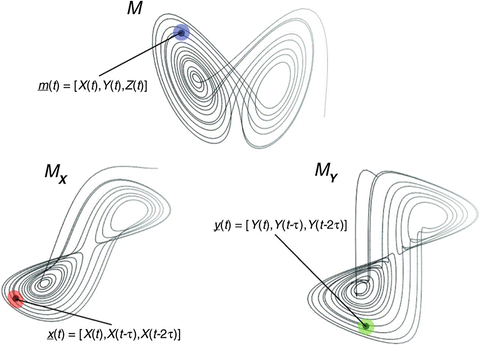
\includegraphics[width=\textwidth]{lecture_5/figs/CCM.png}
\end{figure}
\end{frame}
%=======
\begin{frame}{Метод Local Approximation (LA)}

\begin{enumerate}
    \item Перейдём к векторному представлению временного ряда с помощью векторов задержек и матрицы задержек. В этом методе, однако, удобно изменить порядок следования элементов вектора по времени -- имеем следующее обозначение:
    $$ \mathbf{x}_t = (x_t, x_{t-1}, \dots, x_{t - \tau + 1})^T \in \mathbb{R}^{\tau} $$
    \item Матрица задержек:
    $$\mathbf{X} = 
    \begin{pmatrix}
    \mathbf{x}_{\tau} & \mathbf{x}_{\tau + 1} & \dots & \mathbf{x}_{N-2} & \mathbf{x}_{N-1} & \mathbf{x}_N
    \end{pmatrix} \in \mathbb{R}^{\tau \times (N-\tau + 1)}$$
    
    \item Пусть требуется построить предсказание значения временного ряда $x_{N+1}$. Возьмём предшествующий данному моменту вектор задержек $\mathbf{x}_N$.
    \item Зададимся параметром $S$ и найдём в матрице $\mathbf{X}$ $S$ векторов -- ближайших соседей для $\mathbf{x}_N$ в терминах, например, евклидовой нормы. Обозначим их $\mathbf{x}_{i_1}, \dots, \mathbf{x}_{i_S}$.
    
\end{enumerate}

\end{frame}

%=======
\begin{frame}{Метод Local Approximation (LA)}

\begin{enumerate}
    \item[5.] Предсказание для значения $x_{N+1}$ построим с помощью параметризованной функции $f$: 
    $$ x_{N+1} = f(\mathbf{x}_N | \boldsymbol{\theta})$$
    Например, линейная аппроксимация: $f(\mathbf{x} |\boldsymbol{\theta}) = \theta_0 + \boldsymbol{\theta}_1^T \mathbf{x}$.\\
    Необходимо лишь определить оптимальный набор параметров $\boldsymbol{\theta}$.
    \item[6.] Параметры $\boldsymbol{\theta}$ определим по локальной окрестности вектора $\mathbf{x}_N$ в пространстве векторов задержек:
    $$ \hat{\boldsymbol{\theta}} = \argmin \sum_{s = 1}^S \Big(x_{i_s + 1} - f(\mathbf{x}_{i_s}|\boldsymbol{\theta}) \Big)^2$$
    \item[7.] Окончательно, предсказание для $N+1$-ого значения:
    $$ x_{N+1} = f(\mathbf{x}_N | \hat{\boldsymbol{\theta}})$$
    
\end{enumerate}

\end{frame}
%=======
\begin{frame}{Резюме}
\begin{itemize}
    \item Временной ряд можно аппроксимировать отрезком его ряда Фурье.
    \item Вектор задержек и матрица задержек -- это удобные способы многомерного представления временного ряда.
    \item Метод SSA основан на сингулярном разложении матрицы задержек ряда и, как правило, переходе к её низкоранговому приближению.
    \item Метод LA позволяет предсказывать значения временного ряда по окрестности соответствующего вектора задержек в своём пространстве (идея, схожая с алгоритмом CCM).
\end{itemize}
\end{frame}
\end{document} 